\chapter{Aufbau \gls{programname}}
\label{ch:aufbau_programname}

\section{Architekturbeschreibung}

\gls{programname} ist nach dem \gls{mvp}-Prinzip aufgebaut. Der
\hyperref[subsec:presenter]{Presenter} baut alle anderen Packages auf und
initialisiert diese. Dadurch hat er Zugriff auf jede andere Komponente in \gls{programname},
und kann somit die Kapselung einzelner Komponenten kontrollieren. Dieses Design
trägt zu der Erweiterbarkeit \gls{programname}s bei, da an einer einzigen
Stelle entschieden wird welches Package welches andere Package kennt.
\newline
\newline
Das \hyperref[subsec:service]{service}-Package zusammen mit dem \hyperref[subsec:presenter]{Presenter}
bilden den Controller des \gls{mvc}-Musters. Die Services laufen unabhängig voneinander in
jeweils eigenen Threads und führen bis zur Terminierung des Programms ihre Routinen durch.
Um Services zu kontaktieren werden Commands benötigt, die von einem Executor (ebenfalls ein
Service) ausgeführt werden. So sind die Services als Listener bei allen gemeldet, die ihre
Dienste in Anspruch nehmen wollen (wie z.B. die View, wenn diese Eingaben vom Benutzer erhält).
\newline
\newline
Das \hyperref[subsec:model]{model}-Package wird zur Datenhaltung verwendet. Durch das Service
können am Model Änderungen durchgeführt werden. Falls das Model verändert wird, wird View
darüber in Kenntnis gesetzt (über JavaFX Property Bindings), damit es sich mit den neuen Daten
aktualisieren kann. In unserer Architektur haben wir eine 2:1:1 Beziehung zwischen Model,
View und Controller, da wir einen Live- und einen Replaygraphen anbieten wollen.
\newline
\newline
Zur Darstellung des Models wird das \hyperref[subsec:view]{view}-Package verwendet. Dieses
hat einen eigenen Thread, der dafür zuständig ist, die Graphdaten bei Bedarf neu zu zeichnen,
sowie mithilfe von Interactors die Benutzereingaben als Commands zum Service zu leiten.
\newline
\newline
Zusätzlich gibt es die \hyperref[subsec:command]{command}-, \hyperref[subsec:interaction]{interaction}-
und \hyperref[subsec:util]{util}-Packages, die unserer Variation des \gls{mvc} als Unterstützung dienen.


\begin{figure}[H]
  \centering
  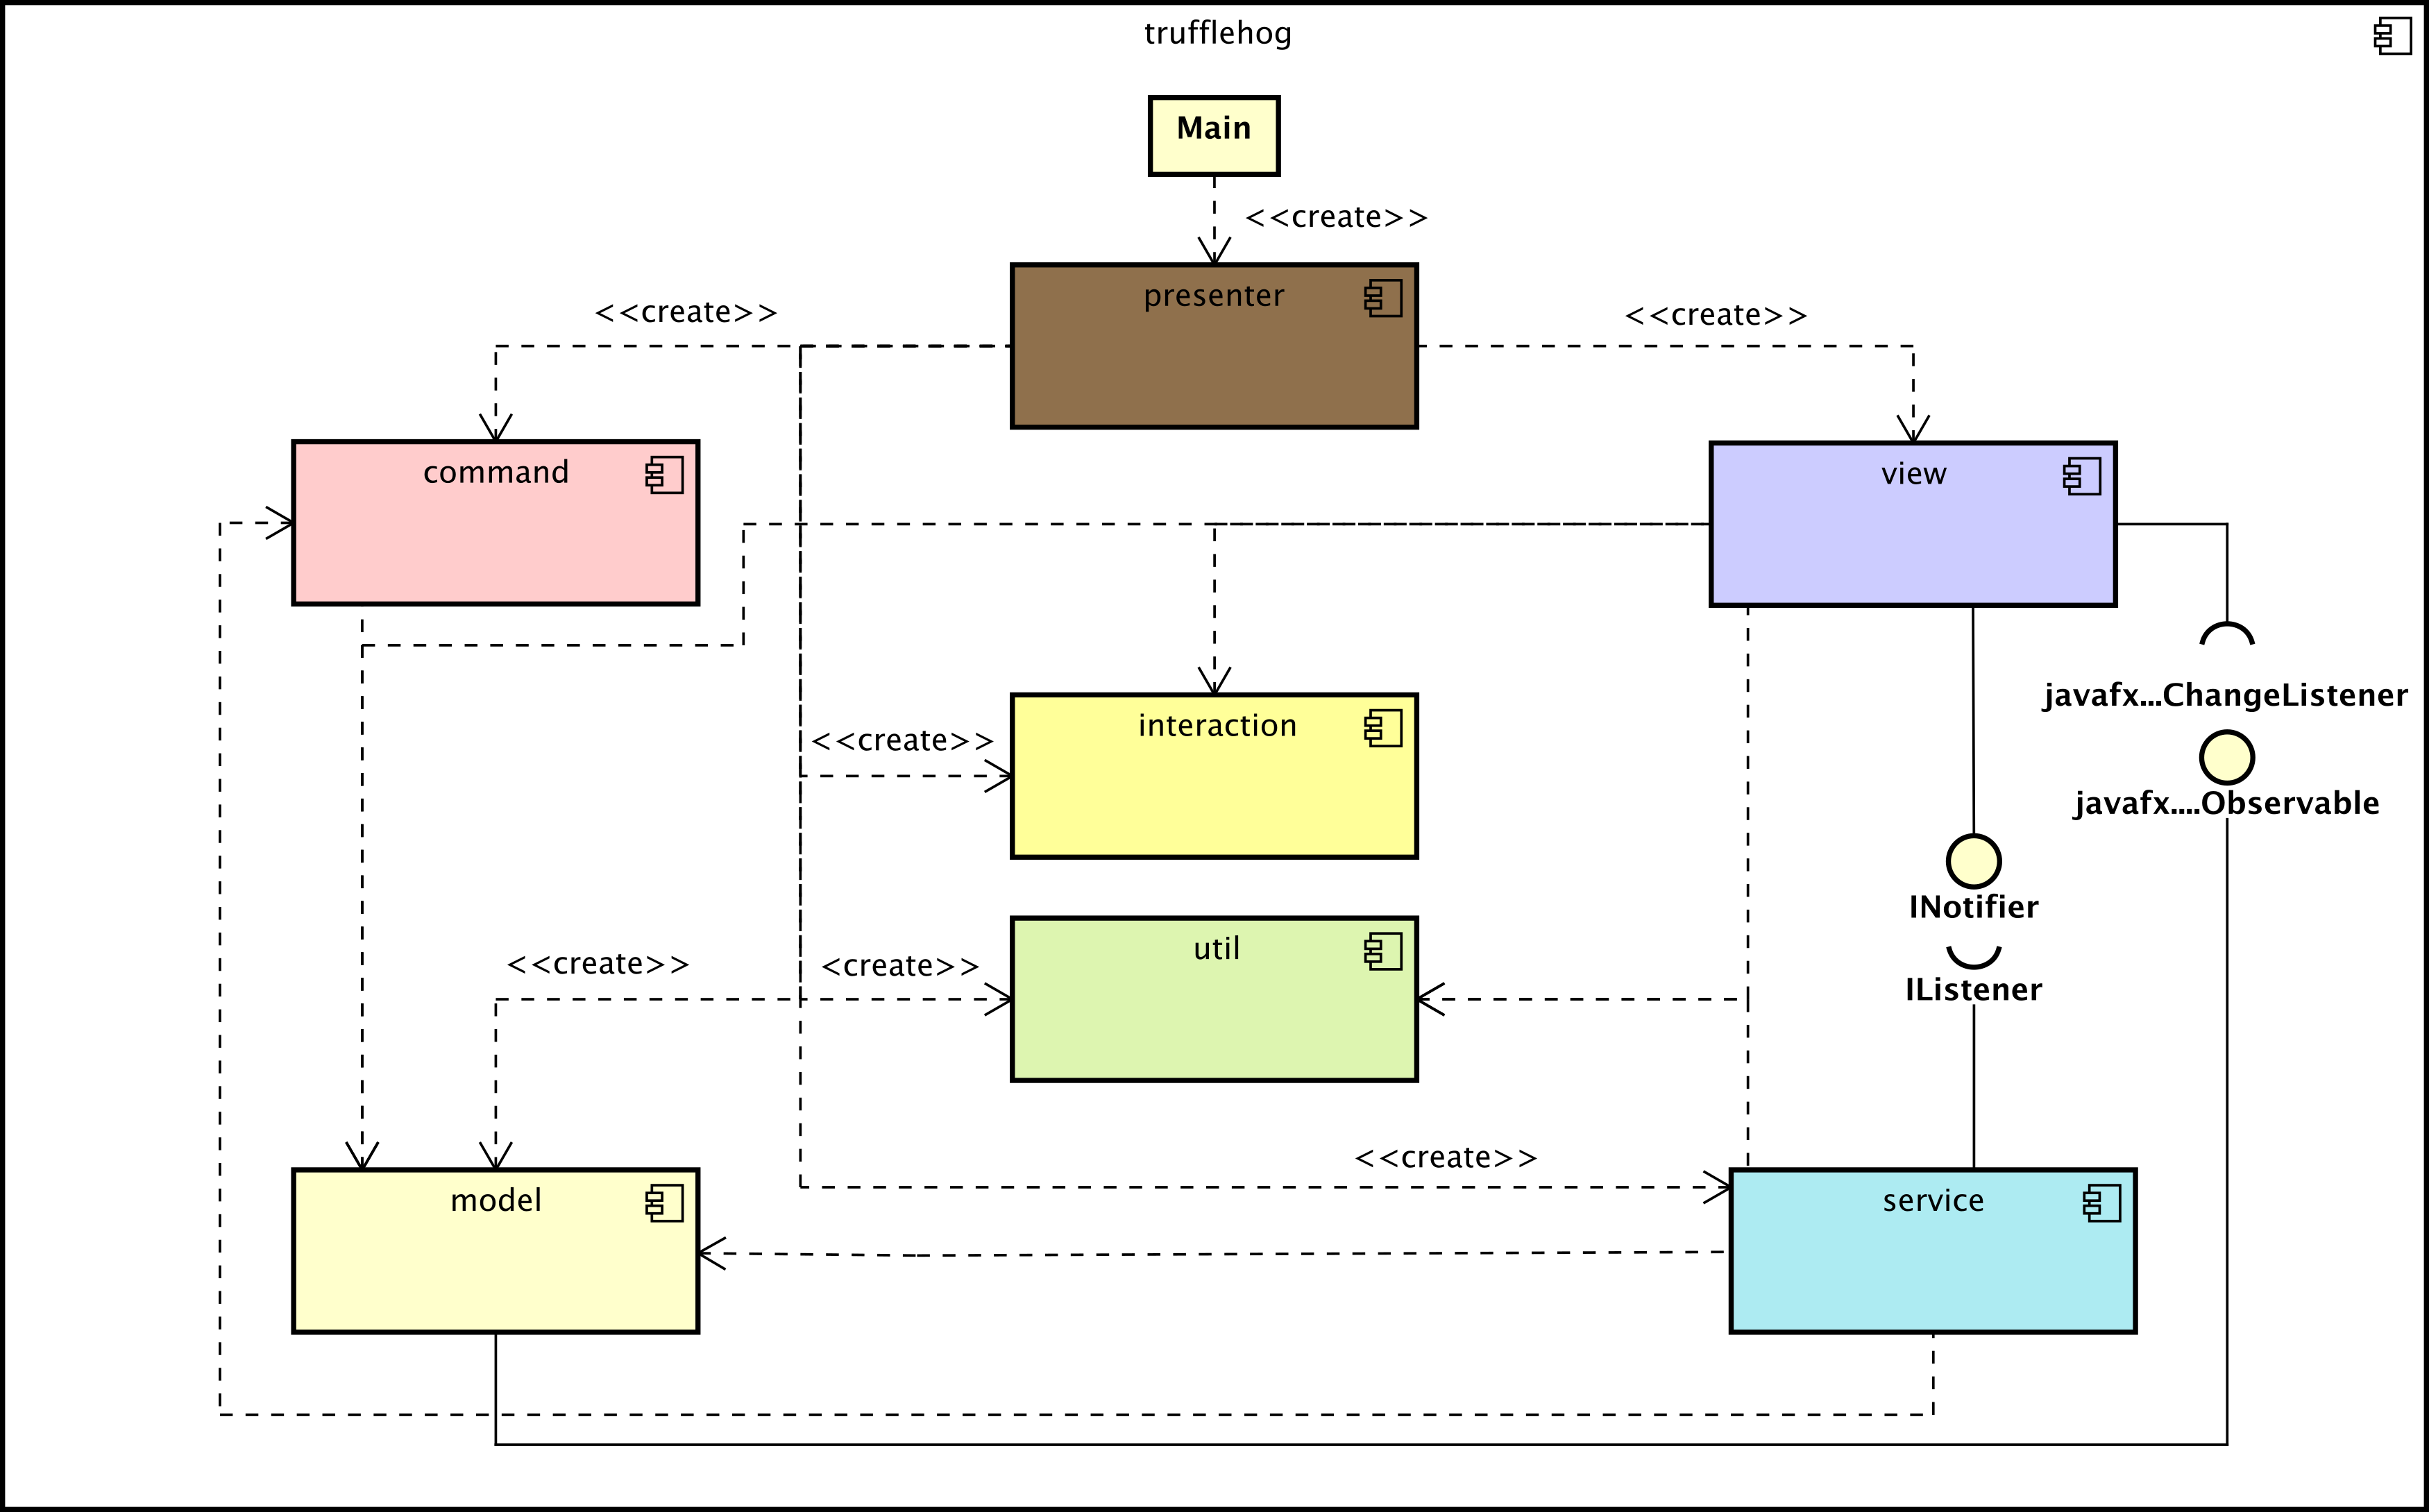
\includegraphics[width=\textwidth]{../diagramimages/trufflehog-component.png}
  \caption{\gls{programname} Packageübersicht}
\end{figure}


\section{Paketbeschreibung}

\subsection{command}
\label{subsec:command}

\begin{figure}[H]
  \centering
  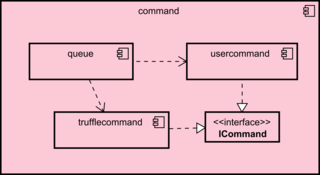
\includegraphics[width=\textwidth]{../diagramimages/command.png}
  \caption{command-Package}
\end{figure}

\medskip
Das command-Package beinhaltet alle Commands, deren Struktur und die Datenstruktur
\textit{CommandQueue}. Ein Command ist eine Befehlssequenz, die auf
dem Model ausgeführt wird. Das heißt, alle Objekte, die das Model irgendwie verändern,
werden als Command gekapselt, sodass die Veränderung auf dem Model
ausgeführt werden kann. Es werden alle empfangene Netzwerkpakete
und Benutzerbefehle als Command gekapselt, da diese direkt das Model beeinflussen
indem sie im Executor ausgeführt werden.
\newline
\newline
Dieses Design hat zwei große Vorteile. Zum einen herrscht eine lose Kopplung zwischen
allen Programmteilen, welche das Model verändern wollen und dem Model selbst, was zur Modularität des ganzen
Programms beiträgt. Zum anderen kann man die Commands speichern und zu einem
späteren Zeitpunkt auf einem Snapshot des Models wieder ausführen, um das originale
Model wiederherzustellen. Weitere Informationen im
\hyperref[subsubsec:replaylogging]{replaylogging}-Package. Des Weiteren bietet dieses
Design den großen Vorteil, dass es hohes Erweiterbarkeitspotential hat. Zum Beispiel
könnte man relativ einfach eine undo- und redo-Funktion in die Commands einbauen, um
zwischen verschiedenen Modelzuständen hin und zurück zu springen, oder generell dem User ermöglichen, Eingaben im Programmablauf durch undo und redo zu kontrollieren. So eine
Funktionalität ist zwar nicht eingeplant, wäre durch dieses Design jedoch nicht schwer zu implementieren.
\newline
\newline
Ein potenzielles Problem, dass auftreten kann, wäre, wenn ein Command zu lange braucht, um
ausgeführt zu werden und so das ganze Programm zum Stillstand kommt.
In dem jetzigen Entwurf wird dieses Problem nicht auftreten, da jeder Command
nur schnelle Befehlssequenze ausführt, welche das System nicht
aufhängen. Wenn jedoch \gls{programname} mal so erweitert wird, dass es doch Commands gibt,
die eine lange Ausführungszeit haben, so sollten diese in seperaten Threads
ausgeführt werden um zu verhindern, dass sich das ganze Programm an einem Command
aufhängt.

Es gibt 2 Arten von Commands, TruffleCommands für die Bearbeitung empfangener
Paketdaten, und UserCommands für die Verwaltung der Benutzeroberflächenbefehle.

      \subsubsection{trufflecommand}
      \label{subsubsec:trufflecommand}

      \begin{figure}[H]
        \centering
        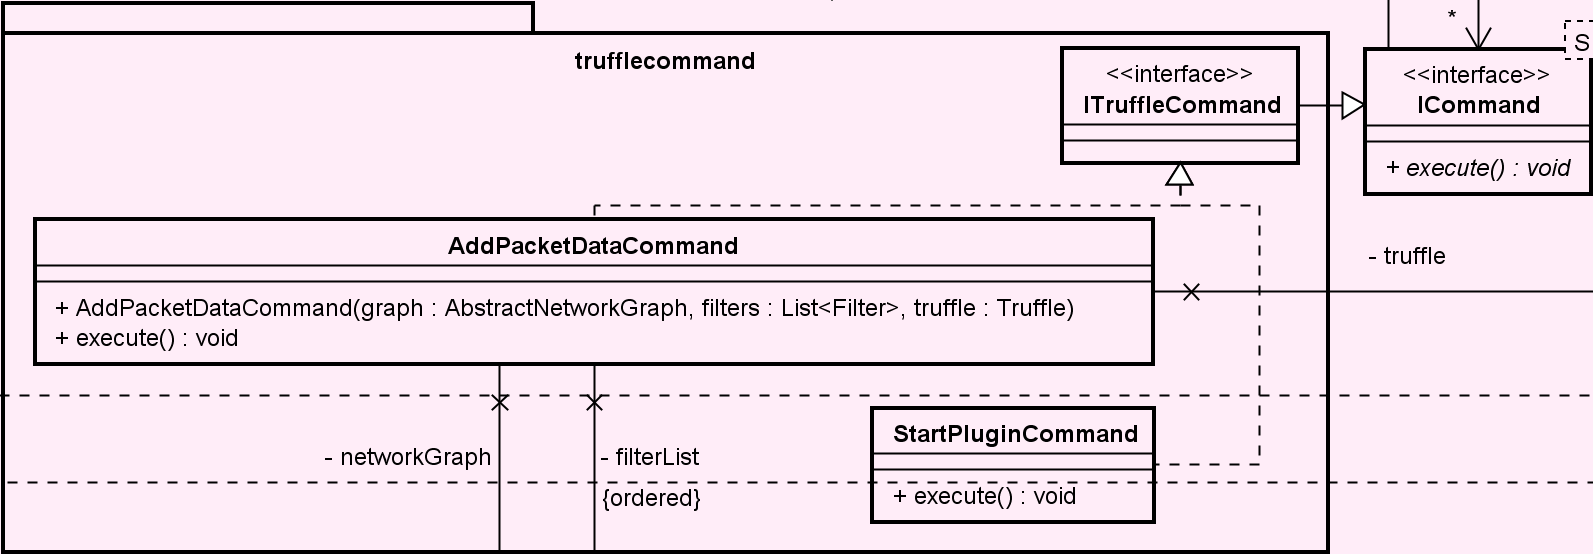
\includegraphics[width=\textwidth]{../diagramimages/trufflecommand.png}
        \caption{trufflecommand-Package}
      \end{figure}

      \medskip
      Jegliche empfangenen \glspl{truffle} vom \gls{praeprozessor} werden zuerst in Java-Objekt-\glspl{truffle} umgewandelt, wie
      im \hyperref[subsubsec:truffleprocessor]{truffleprocessor}-Package erleutert. Dort
      werden die erzeugten Java-\glspl{truffle} in ein Command gesteckt und per \gls{observerpattern}
      wie im \hyperref[subsec:util]{util}-Package beschrieben an alle Interessenten, also die \gls{listener}, verschickt.
      \newline
      \newline
      Es gibt nur einen Command-Typen für die empfangen \gls{truffle}-\glspl{paket}, nämlich den
      AddPacketDataCommand. Diese Entscheidung wurde getroffen, um das Programm einfach
      zu halten. Commands wie AddNode oder AddEdge sind überflüßig, da diese leicht aus
      dem Inhalt des \glspl{truffle} geschlossen werden können.
      \newline
      \newline
      Der PluginNotRunningCommand wird genau dann vom truffleprocessor verschickt, wenn sich \gls{programname}
      nicht mit \gls{sppname} oder einem äquivalenten Plugin verbinden konnte. Wir
      haben die Funktionalität, dass \gls{programname} automatisch \gls{sppname} startet,
      aufgegeben, um die beiden Programme unabhängiger zu gestalten, und um dem Benutzer
      mehr Freiheit, beispielsweise bei der \gls{praeprozessor}enwahl, zu geben.

      \subsubsection{usercommand}
      \label{subsubsec:usercommand}

      \begin{figure}[H]
        \centering
        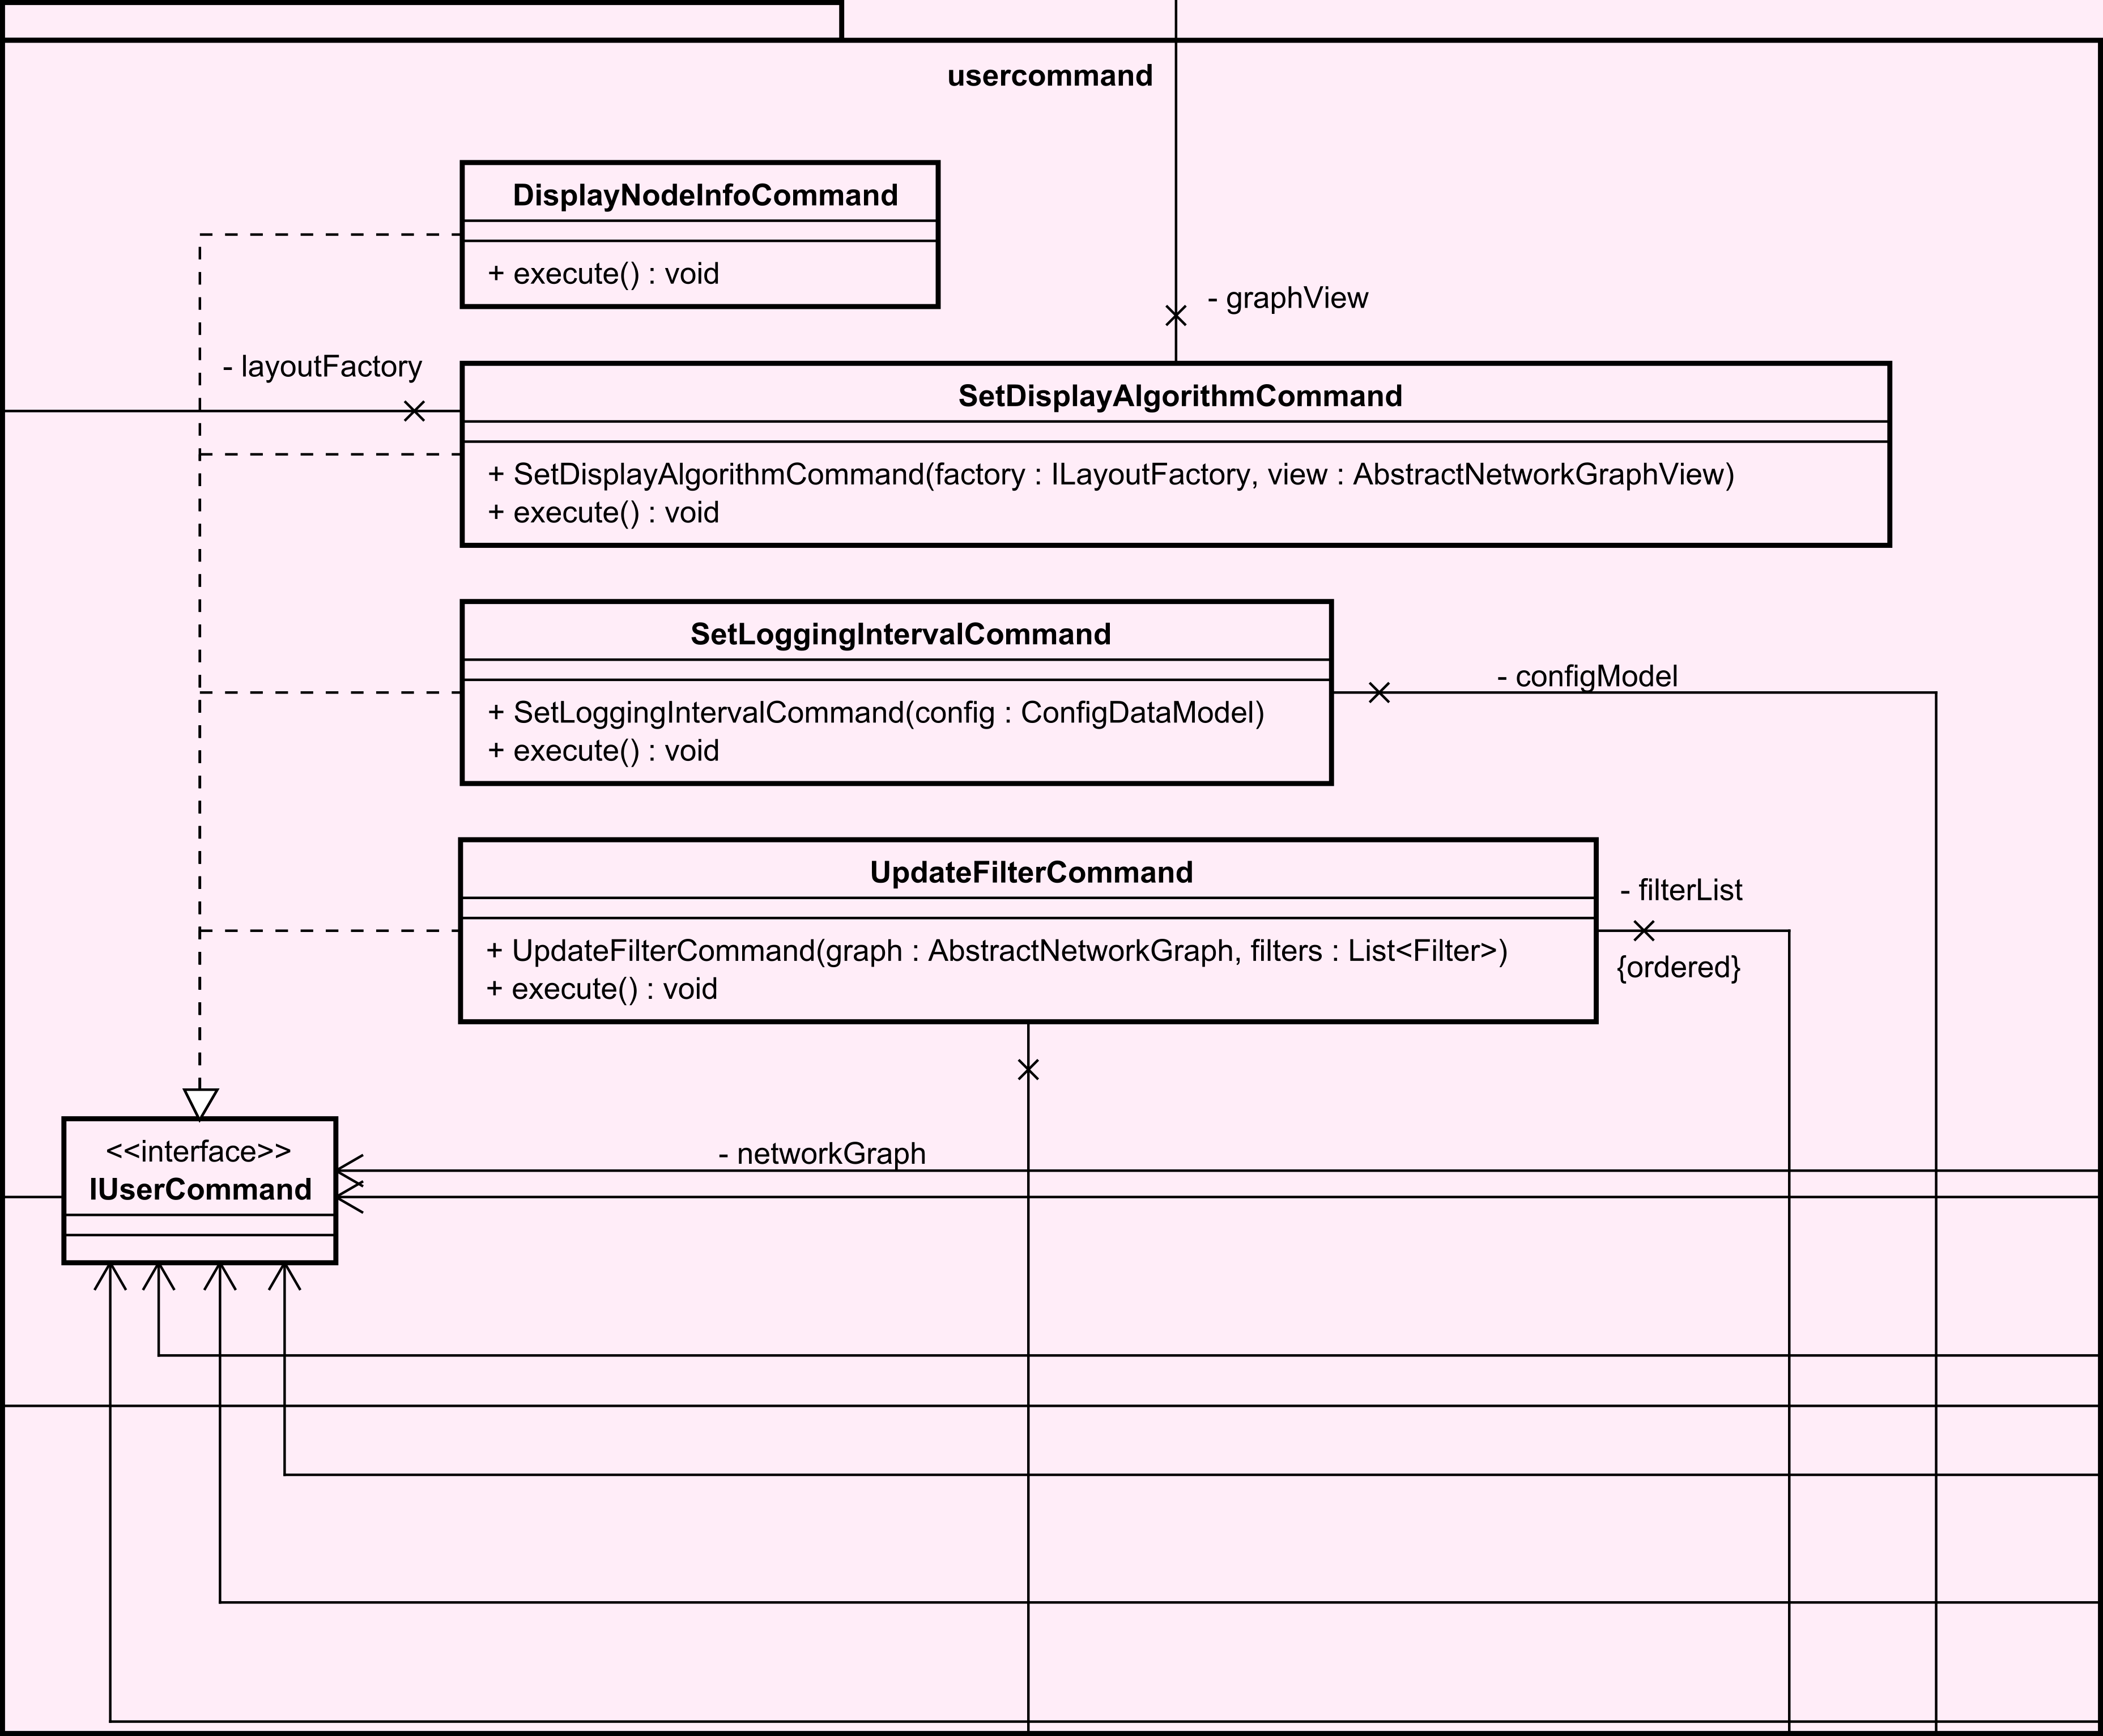
\includegraphics[width=\textwidth]{../diagramimages/usercommand.png}
        \caption{usercommand-Package}
      \end{figure}

      \medskip
      Wenn der Benutzer eine \gls{gui}-Aktion startet, die das Model beeinflusst,
      wird ein entsprechender Command an alle \gls{listener} durch das \gls{observerpattern}, wie im
      \hyperref[subsec:util]{util}-Package beschrieben, verschickt. Für jede mögliche
      \gls{gui}-Aktion, welche das Model beeinflusst, gibt es einen passenden Command.
      Diese werden in den ViewControllern aus dem \hyperref[subsec:view]{view}-Package, wieder nach \gls{observerpattern},
      an den Executor verschickt.

      \subsubsection{queue}
      \label{subsubsec:queue}

      \begin{figure}[H]
        \centering
        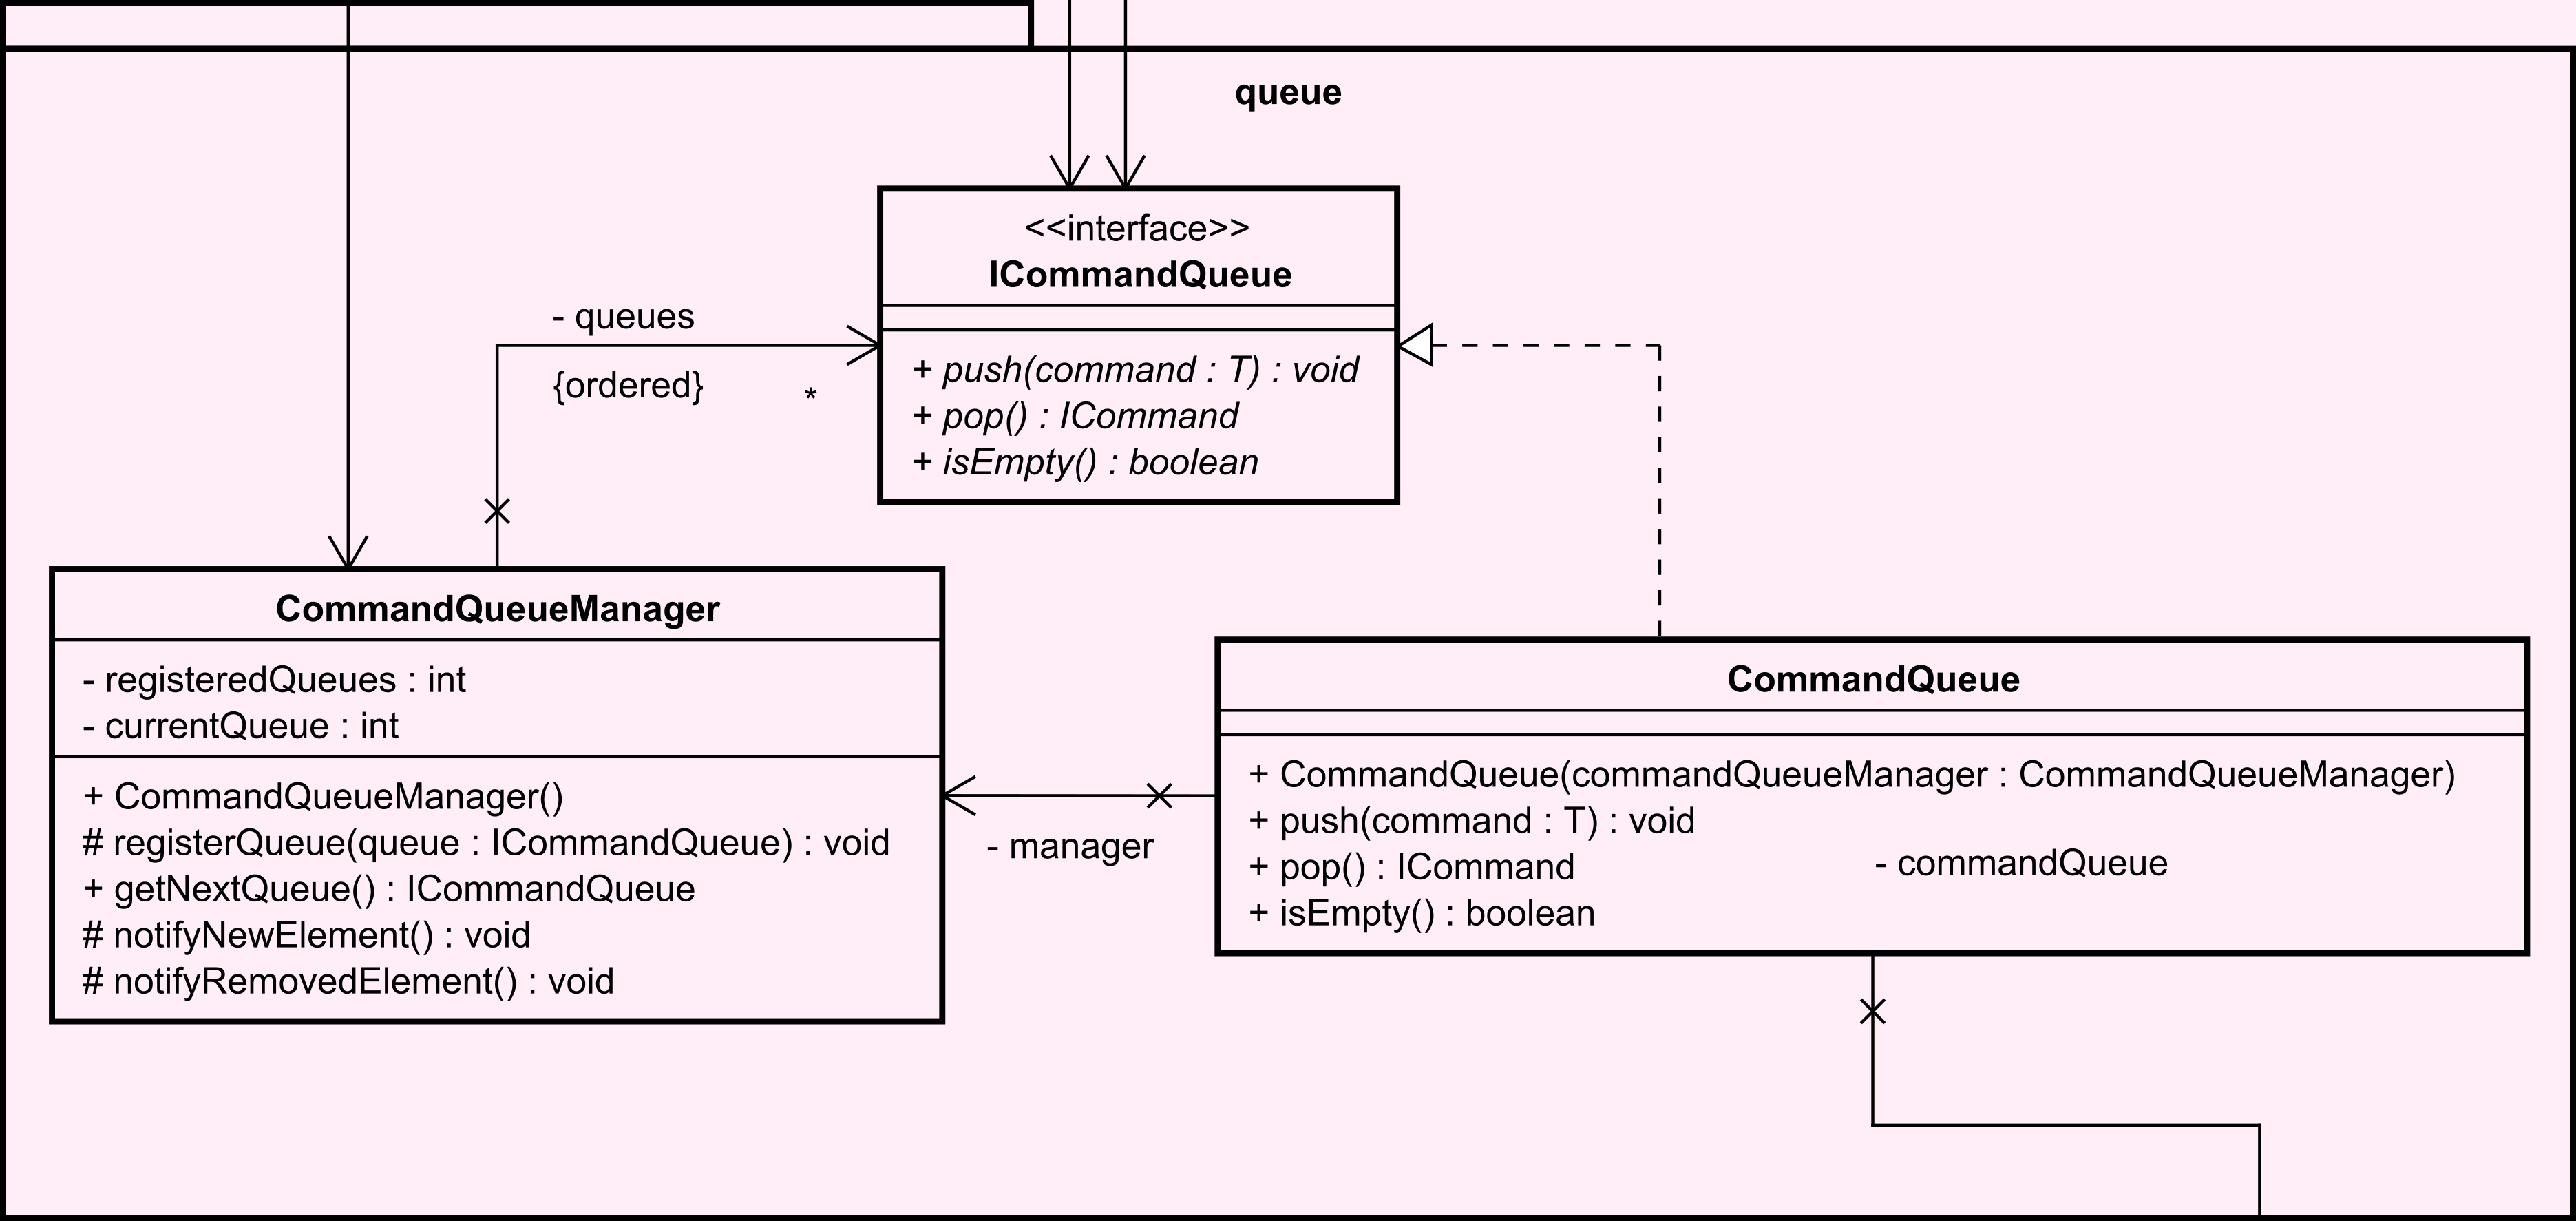
\includegraphics[width=\textwidth]{../diagramimages/queue.png}
        \caption{queue-Package}
      \end{figure}

      \medskip
      Die Commands, welche beispielsweise der Executor abarbeiten soll, werden in
      einer passenden Datenstruktur zwischengespeichert. Es sind ggf. mehrere
      tatsächliche Queues vorhanden, was nach einem Manager verlangt, um nach dem
      Round-Robin-Prinzip faire Abarbeitung zu ermöglichen. Diese CommandQueue
      ist das empfangende Ende des \gls{observerpattern}s an mehreren Stellen unseres
      Programms. Bei Aktualisierung durch einen \gls{notifier} geht dieser alle
      seine \gls{listener} durch und fügt bei jedem in genau einer diese
      CommandQueue das neue Command-Objekt ein. Die Implementierung der Queues
      als BlockingQueue ermöglicht in diesem Fall die Kommunikation zwischen Threads.


\subsection{service}
\label{subsec:service}

\begin{figure}[H]
  \centering
  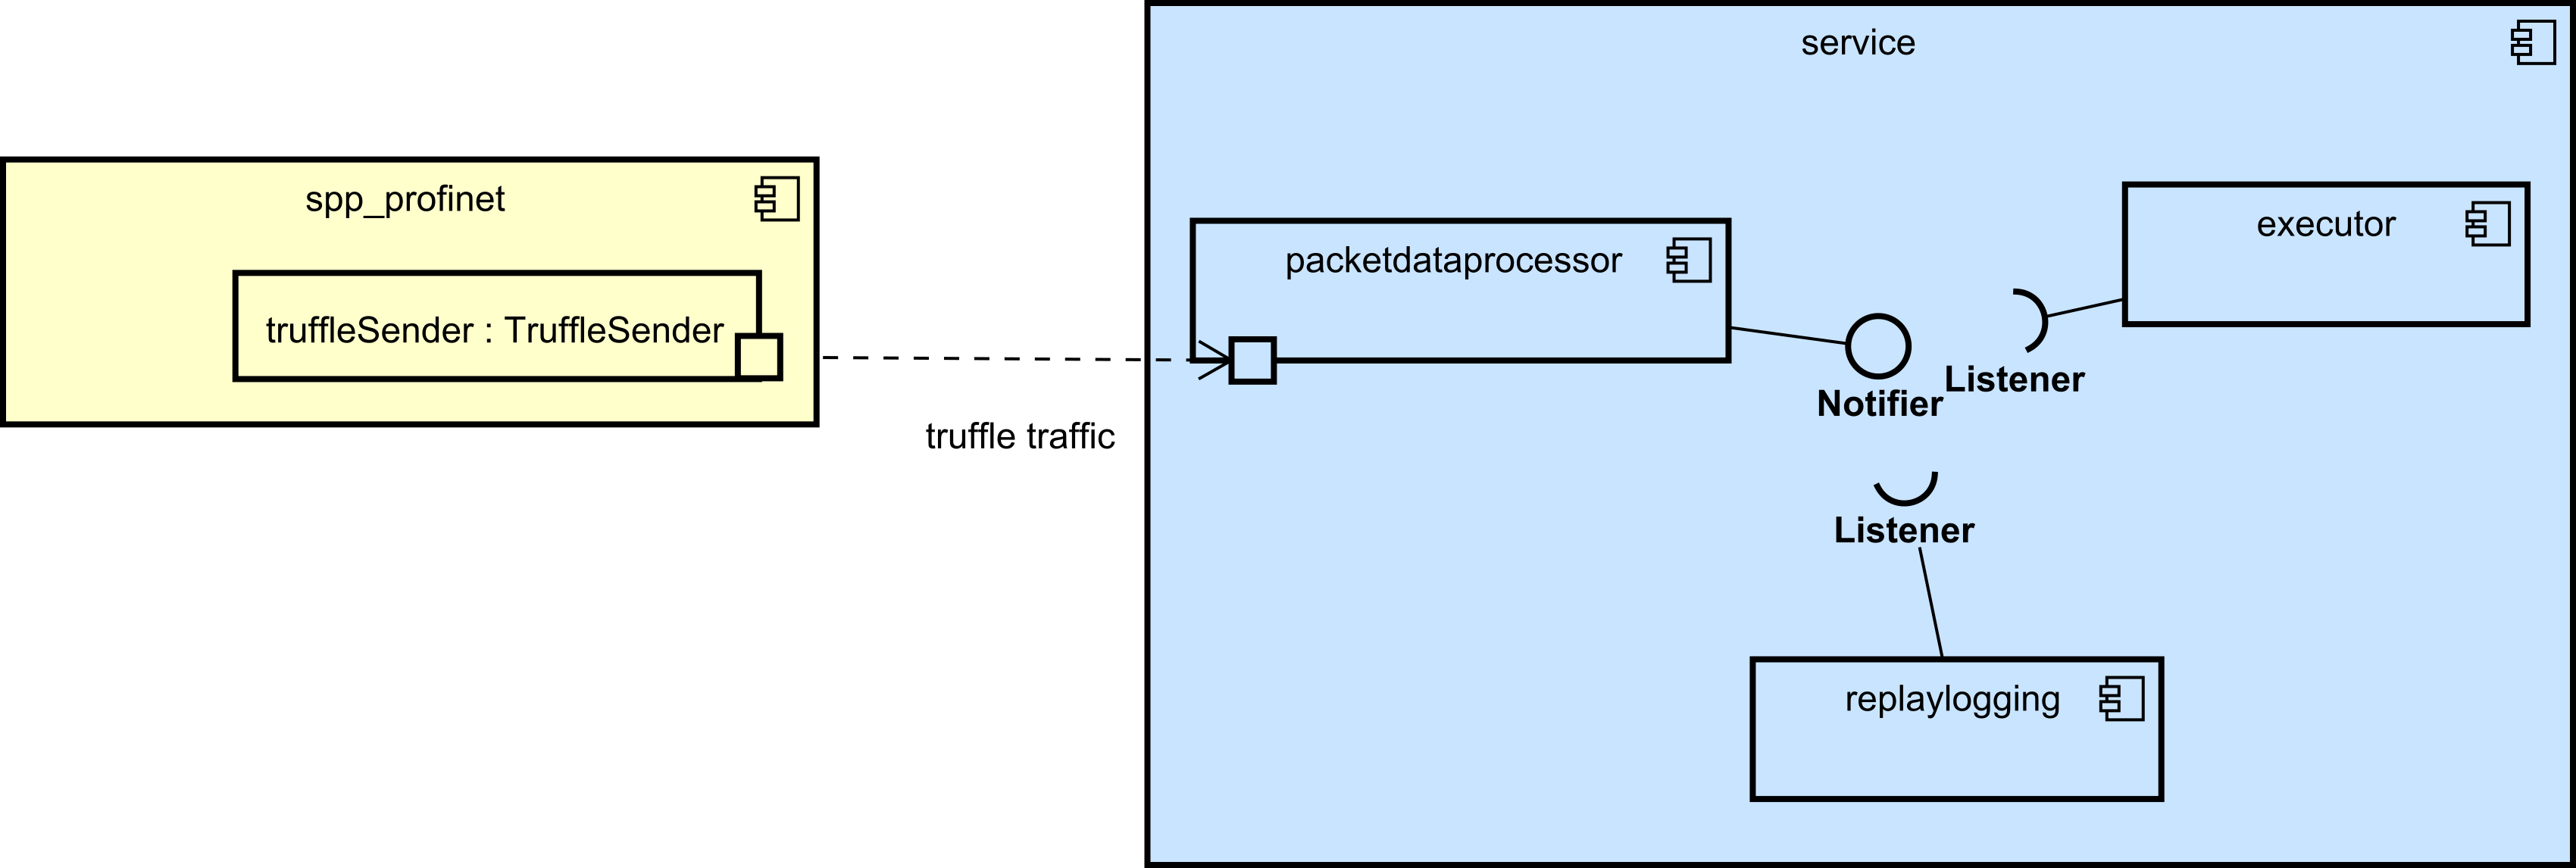
\includegraphics[width=\textwidth]{../diagramimages/service.png}
  \caption{service-Package}
\end{figure}

\medskip
Im service-Package befinden sich alle durchlaufenden Threads von \gls{programname},
mit Ausnahme vom \hyperref[subsec:view]{view}, das ein eigenes Package zur verzögerungsfreien Darstellung ist, und dem
main-Thread. Jedes Unterpackage kapselt dabei genau eine selbständig laufende Funktionalität, meist eine pro Thread. In den folgenden Abschnitten ist erklärt, was genau die Unterpackages packetdataprocessor, replaylogging und executor machen.

    \subsubsection{packetdataprocessor}
    \label{subsubsec:truffleprocessor}

    \begin{figure}[H]
      \centering
      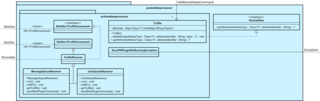
\includegraphics[width=\textwidth]{../diagramimages/packetdataprocessor.png}
      \caption{packetdataprocessor-Package}
    \end{figure}

    \medskip
    Der packetdataprocessor-Service läuft konstant im Hintergrund, in einem eigenen Thread,
    und empfängt die im \gls{sppname} erstellten Truffles.
    Diese packt er in ein Java-Truffle-Objekt, welches dann wiederum von dem
    \textit{TruffleReciever} in ein Command gesteckt wird. Da der \textit{TruffleReciever}
    auch ein \gls{notifier} ist, verschickt er den Command auch gleich an
    alle registrierten \gls{listener}, sodass der CommandExecutor die bekommt wo die Commands
    als nächstes auf dem Model angewandt werden.

    \subsubsection{replaylogging}
    \label{subsubsec:replaylogging}

    \begin{figure}[H]
      \centering
      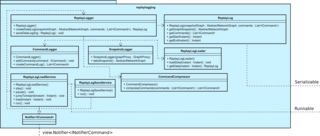
\includegraphics[width=\textwidth]{../diagramimages/replaylogging.png}
      \caption{replaylogging-Package}
    \end{figure}

    \medskip
    Der replaylogging-Service besteht aus 2 Hauptaufgaben, die jeweils ihren eigenen Thread haben.
    Der erste ist der \textit{ReplayLogSaveService} und kümmert sich um das speichern das aktuellen
    Graphen. Der zweite ist der \textit{ReplayLogLoadService} und kümmert sich um das
    wiederherstellen eines gespeicherten Graphen.
    \newline
    \newline
    Der \textit{ReplayLogSaveService} läuft konstant im Hintergrund und empfängt alle
    vom \textit{TruffleReciever} verschickten Commands. Diese werden alle X
    Sekunden (vom Benutzter festlegbar) komprimiert und in eine Liste gepackt.
    Komprimiert heißt, dass viele Commands, die das selbe tun, in ein Command
    gepackt werden. Zusätzlich zu den Commands wird auch noch ein Snapshot
    von dem aktuellen Graphen gemacht, der dann zusammen mit der erstellten
    Command-Liste in ein ReplayLog-Objekt getan wird. Dieses
    ReplayLog-Objekt wird dann von Java serialisiert und gespeichert.
    \newline
    \newline
    Diese Logs können zu einem späteren Zeitpunkt wieder geladen werden um den
    Graphen wiederherzustellen. Dazu ist der \textit{ReplayLogLoadService} da. Wenn
    der User die Replayfunktion aktiviert, fängt der ReplayLogLoadService an die
    ReplayLogs zu laden. Dann wird in der view der Snapshotgraph angezeigt
    und die gespeicherten Commands aus dem ReplayLog werden auf
    diesem Snapshot angewandt. Der ReplayLogLoadService kontrolliert somit die
    Wiedergabe des alten Graphen und kann sogar hin und her zwischen Snapshots
    springen (momentan nicht zwischen einzelnen Commands, da dieses keine undo-
    und redo-Funktion besitzten).
    \newline
    \newline
    Der ReplayLogLoadService läuft in seinem eigenen Thread, weil er sich darum
    kümmert das immer genügend Daten im Speicher liegen. In anderen Worten, er
    buffert die Replaylogs vor damit sich der Graph bei dem Benutzter flüssig
    abspielt.

    \subsubsection{executor}
    \label{subsubsec:executor}

    \begin{figure}[H]
      \centering
      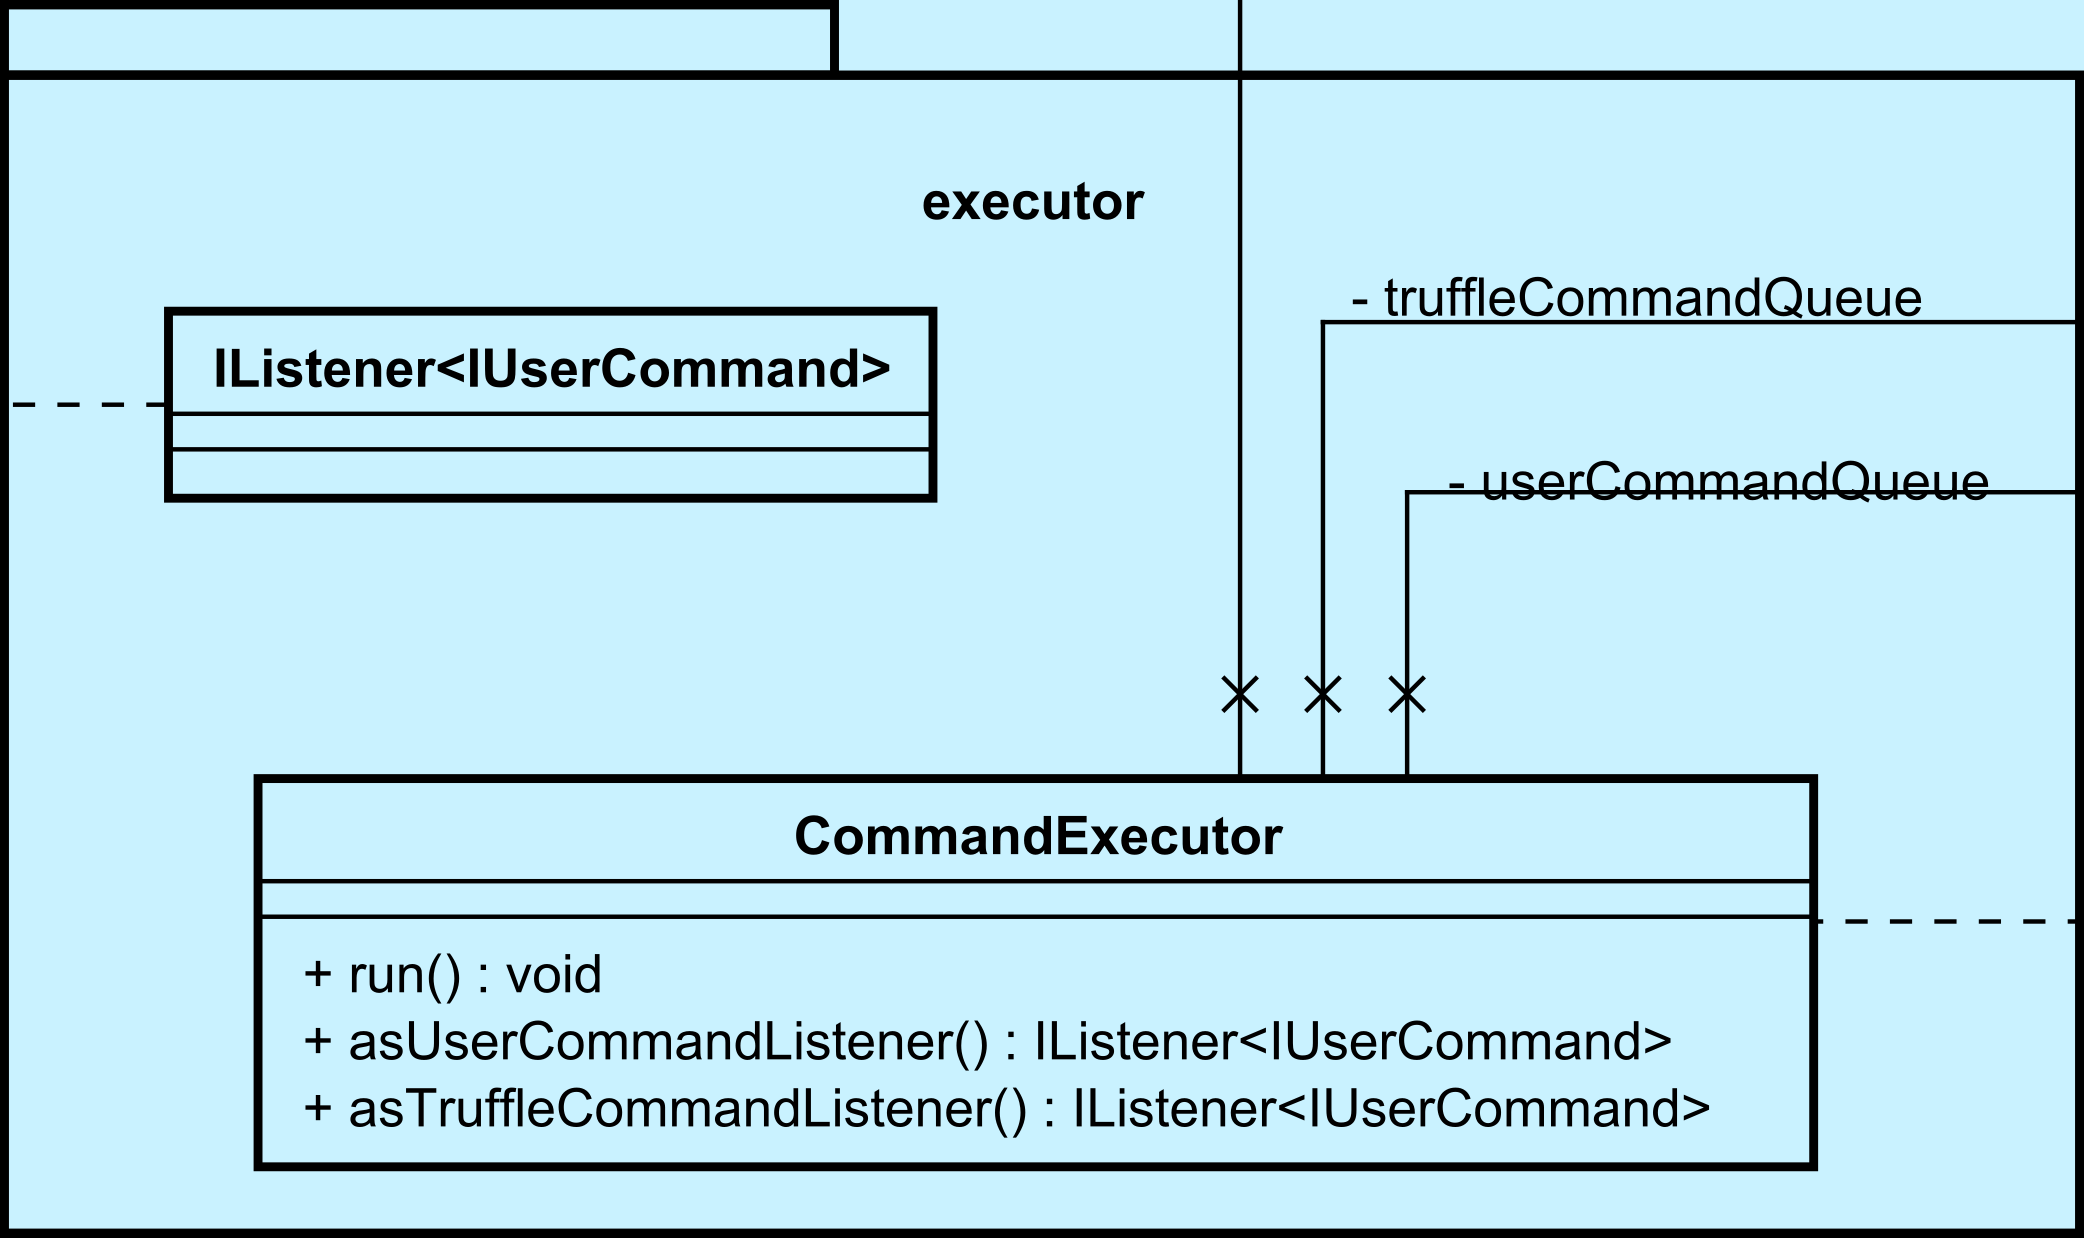
\includegraphics[width=\textwidth]{../diagramimages/executor.png}
      \caption{executor-Package}
    \end{figure}

    \medskip
    Der executor-Service läuft auch wieder konstant im Hintegrund in seinem
    eigenen Thread. Er ist ein \gls{listener} der sowohl bei dem TruffleReciever aus dem
    \hyperref[subsubsec:packetdataprocessor]{packetdataprocessor}-Package als
    auch bei den view-Controllern aus dem \hyperref[subsec:view]{view}-Package
    registriert ist. D.h. er bekommt, wie das \hyperref[subsubsec:replaylogging]{replaylogging},
    alle \hyperref[subsubsec:trufflecommand]{TruffleCommands} und führt diese
    dann auf dem aktuellen Model aus.
    \newline
    \newline
    In \gls{programname} gibt es zwei Instanzen vom Executor. Die erste bearbeitet
    den aktuellen Graphen und die zweite bearbeitet die Snapshot-Instanz, falls
    eine existiert. So kann der aktuelle Graph auf dem neusten Stand bleiben, während
    gleichzeitig der Benutzter einen alten Graphen aus
    ReplayLogs rekonstruiert anschaut.


\subsection{presenter}
\label{subsec:presenter}

\begin{figure}[H]
  \centering
  \includegraphics[width=0.6\textwidth]{../diagramimages/presenter.png}
  \caption{presenter-Package}
\end{figure}

\medskip
Der presenter ist für den Aufbau von \gls{programname}, also das
Initialisieren, Instanziieren und Referenzieren aller Programmelemente zuständig.
Er ist sozusagen der ``glue code'' von \gls{programname}.
Er wird im main-Thread von der main-Klasse erzeugt und ruft alle Konstruktoren auf.
In anderen Worten baut er \gls{programname} auf.

\subsection{util}
\label{subsec:util}

\begin{figure}[H]
  \centering
  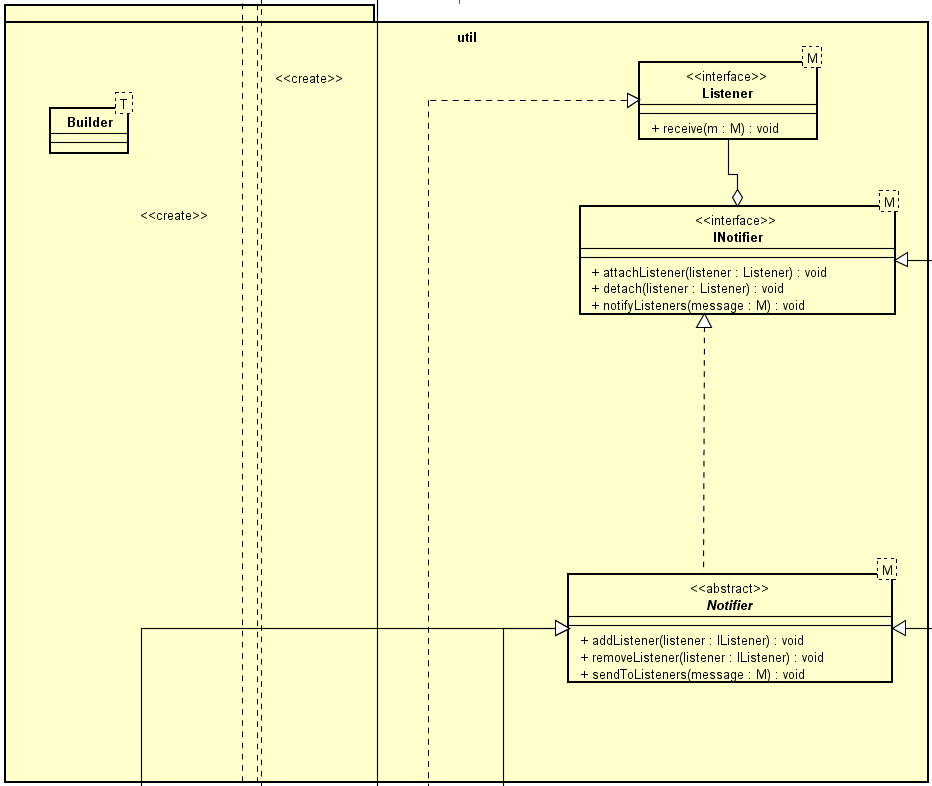
\includegraphics[width=\textwidth]{../diagramimages/util.png}
  \caption{util-Package}
\end{figure}

\medskip
Im util-Package befinden sich Klassen, die komplett von \gls{programname} abgekoppelt
sind. D.h., sie werden nur als Ressource wie eine Liste benutzt und nehmen keinen
Bezug auf das Programm. Konkret befinden sich drei Klassen im util-Package, die alle zusammen eine
Variation des \gls{observerpattern}s realisieren. Der \textit{Notifier} ist dazu da,
ein beliebiges Objekt zu verschicken, deshalb der Generic. Er ist das Subjekt aus
dem \gls{observerpattern}.
\newline
\newline
Der \textit{INotifier} existiert für den Fall, dass ein
Objekt ein Notifier sein muss, aber nicht Notifier vererben kann, weil er
schon eine andere Klasse beerbt. Dieses Problem tritt beispielsweise im
\hyperref[subsec:view]{view}-Package auf, wo viele Klassen \gls{gui}-Aktionen als Commands
gekapselt an den Executor verschicken und gleichzeitig JavaFX Klassen beerben müssen.
Um dieses Problem zu lösen, implementieren diese Klassen das INotifer-Interface
und haben ein Hilfsobjekt, das Notifier vererbt um somit die gewünschte Funktionalität zu
bieten.
\newline
\newline
Der \textit{IListener} ist der Beobachter aus dem \gls{observerpattern}. Hier ist nicht
viel variiert worden, mit Ausnahme der receive-Methode, bei der ein Parameter eingeführt
wurde, damit der Listener das verschickte Objekt des \gls{notifier}s empfangen und darauf arbeiten kann. Zu diesem Zweck existiert erneut ein Generic.
\newline
\newline
Dieses \gls{observerpattern} verwaltet das Verschicken und Empfangen von Commands in
\gls{programname}. In anderen Worten, jede Klasse, die Commands verschickt, ist ein
\gls{notifier}, und jede Klasse, die Commands empfängt, ist ein \gls{listener}. Dieses Design
hat große Vorteile, da die Sender und die Empfänger komplett voneinander abgekoppelt
sind. Der \hyperref[subsec:presenter]{Presenter} registriert die \gls{listener} bei Programmstart
bei den \gls{notifier}n. Somit kennt der \gls{listener} nicht seinen \gls{notifier}, und der
\gls{notifier} weiß nicht, was sich hinter einem \gls{listener} versteckt. Durch diese lose
Kopplung ist es einfach, \gls{programname} um einen zusätzlichen Service zu erweitern,
da kein Service wirklich von einem anderen abhängt.
\newline
\newline
Ein Beispiel dieser losen Kopplung kann man zwischen dem
\hyperref[subsubsec:packetdataprocessor]{packetdataprocessor}-Package, dem
\hyperref[subsubsec:executor]{executor}-Package und dem
\hyperref[subsubsec:replaylogging]{replaylogging}-Package finden. Hier erstellt
der Truffleprocessor neue Commands, die sowohl von dem Executor als auch von dem
ReplayLogSaveService empfangen werden. Obwohl die drei Packages sehr viel
miteinander zu tun haben, kennen sie sich gegenseitig nicht. Dieses Design
trägt zur Modularität von \gls{programname} bei.


\begin{frame}{presenter}
  \begin{figure}
    \centering
    \includegraphics[width=\textwidth]{./images/presenter.png}
  \end{figure}
\end{frame}

\begin{frame}{presenter}
  \begin{itemize}[<+->]
    \item Aufgaben
      \begin{itemize}
        \item Wichtig bei Programmstart, Aufruf in der main Methode
        \item Instanziieren und Initialisieren der Programmelemente
        \item Aufrufen der Services
        \item Übergeben der Abhängigkeiten und Bestimmung der Nutzerrelationen
      \end{itemize}
      \item Entwurfsentscheidungen
        \begin{itemize}
          \item Erster Teil der Variation des Controllers
          \item Entkopplung von Initialisierung und dauerhaften Programmabläufen
          \item Leicht änderbarer Programmaufbau
        \end{itemize}
  \end{itemize}
\end{frame}

\begin{frame}{model}
  \begin{figure}
    \centering
    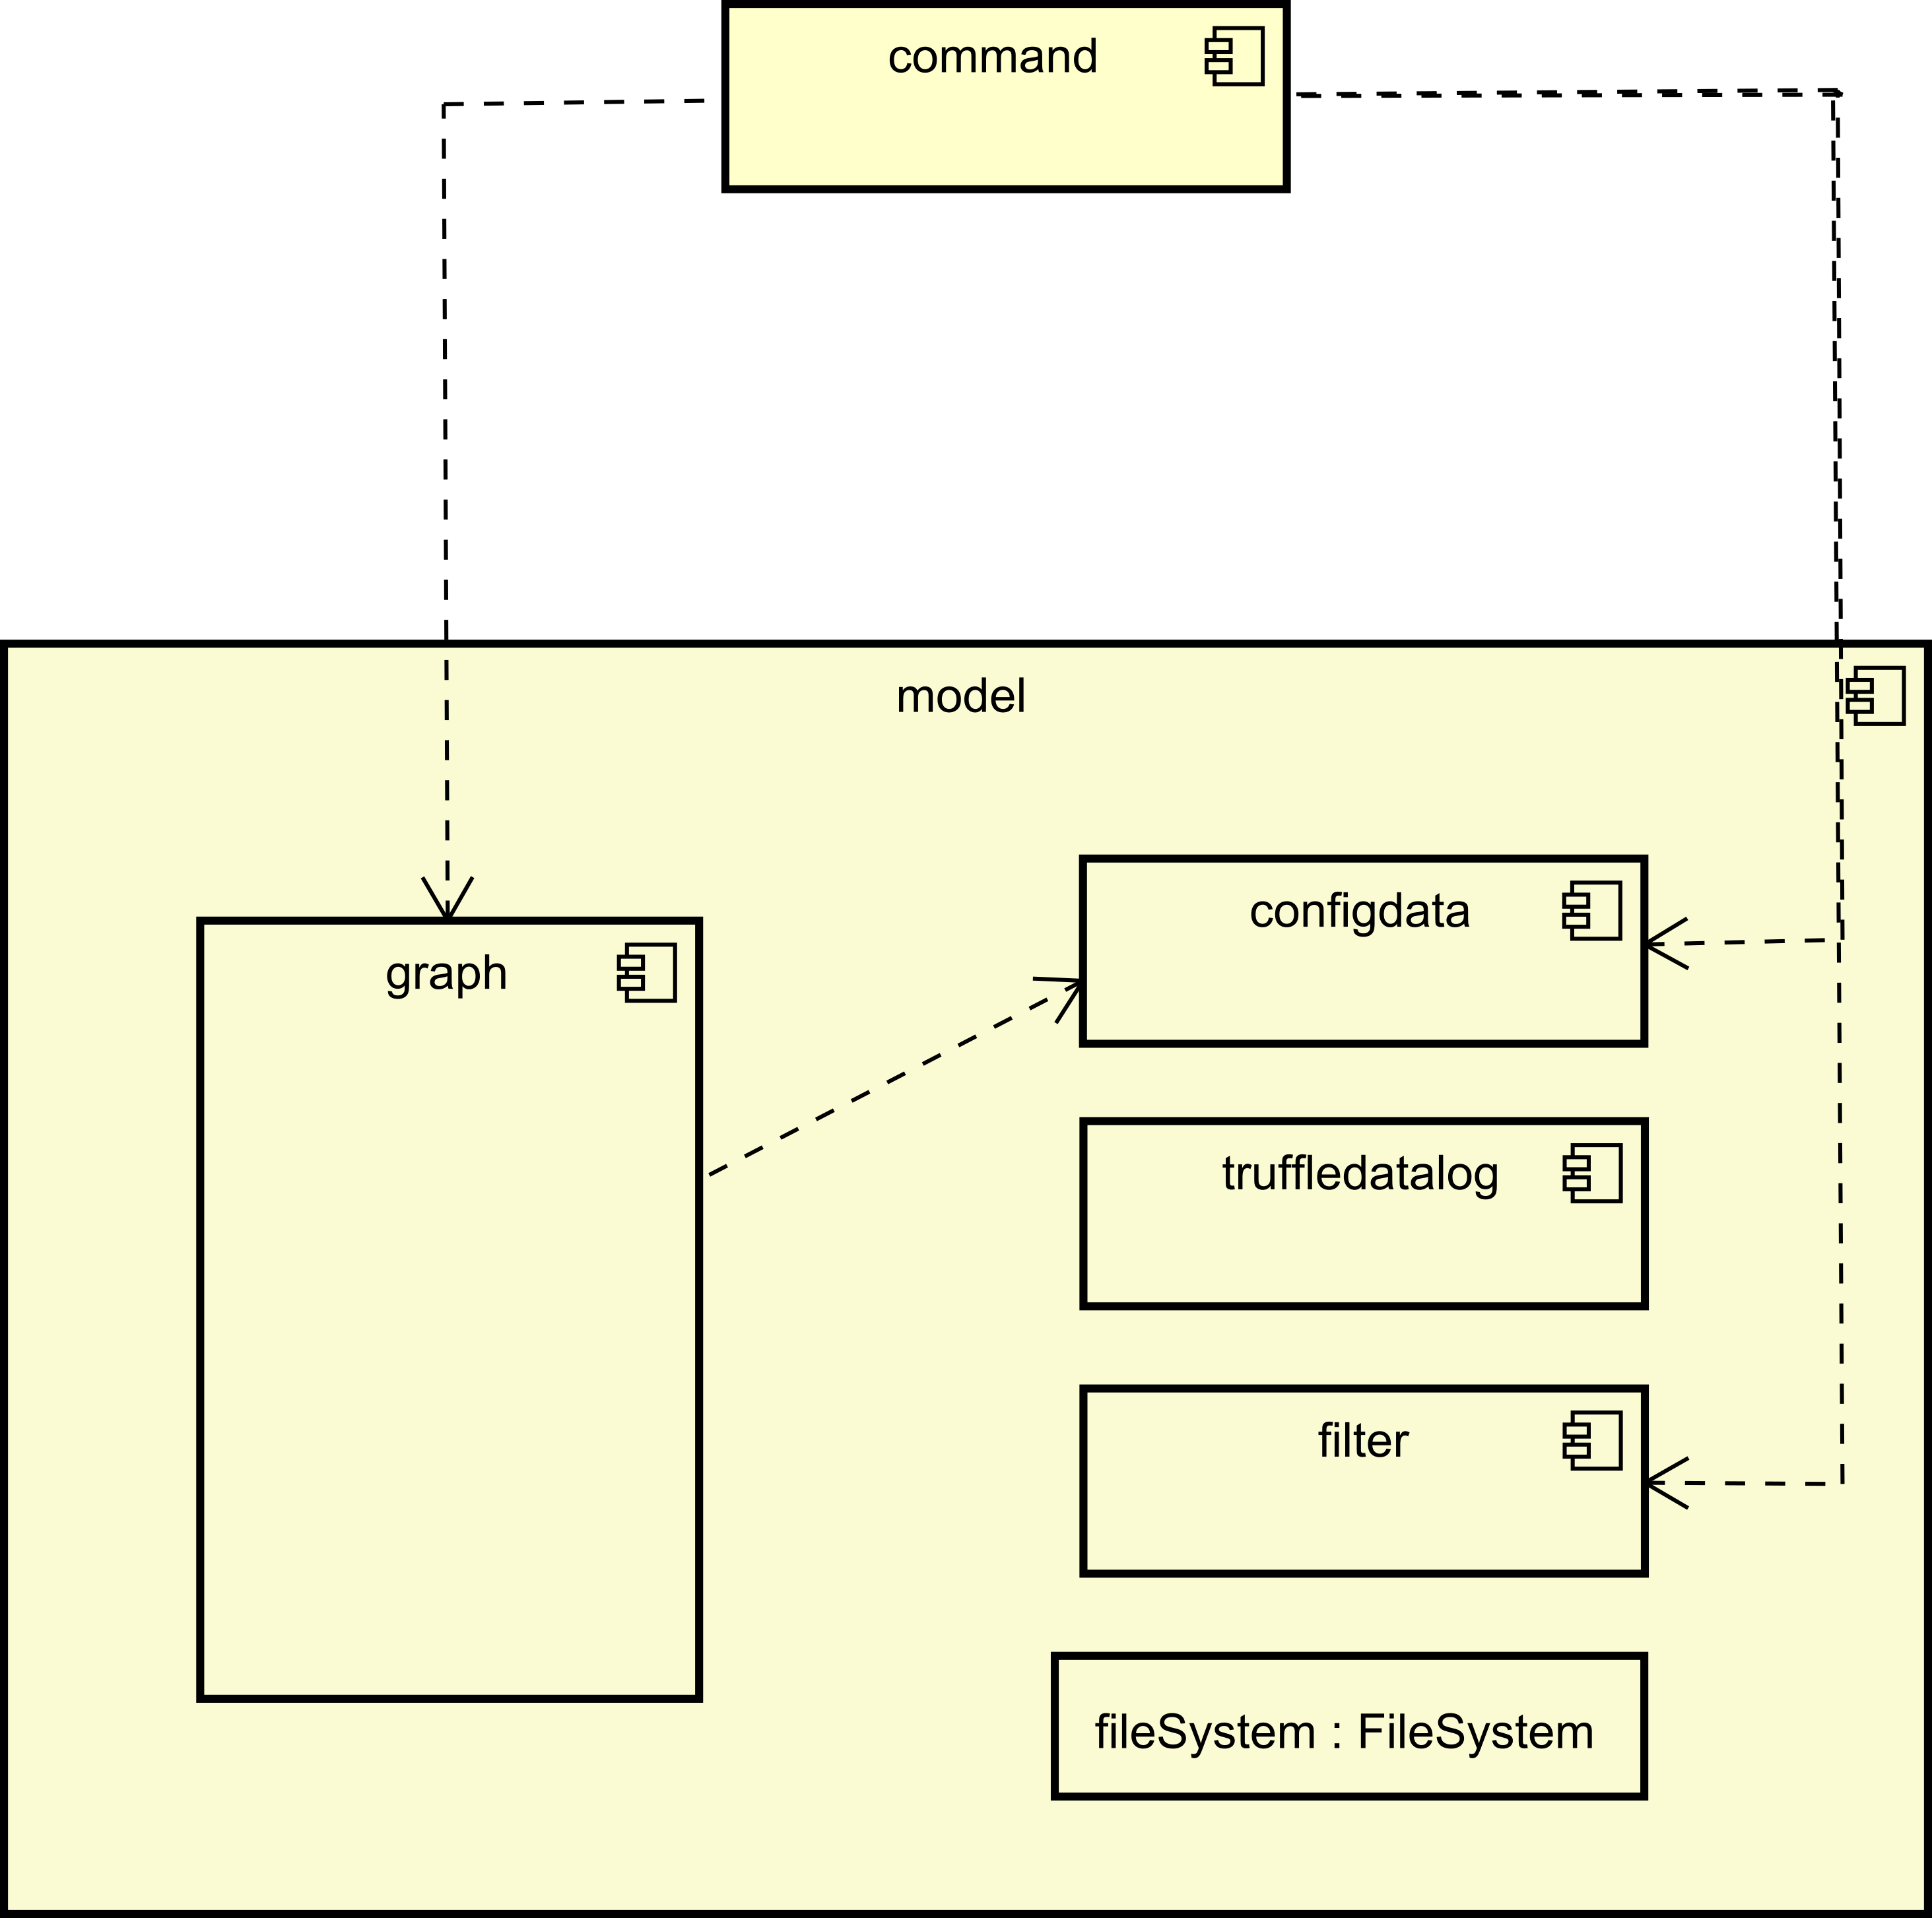
\includegraphics[width=0.6\textwidth]{./images/model.png}
  \end{figure}
\end{frame}

\begin{frame}{model - Graph Selektion im Graph Paket}
  \begin{figure}
    \centering
    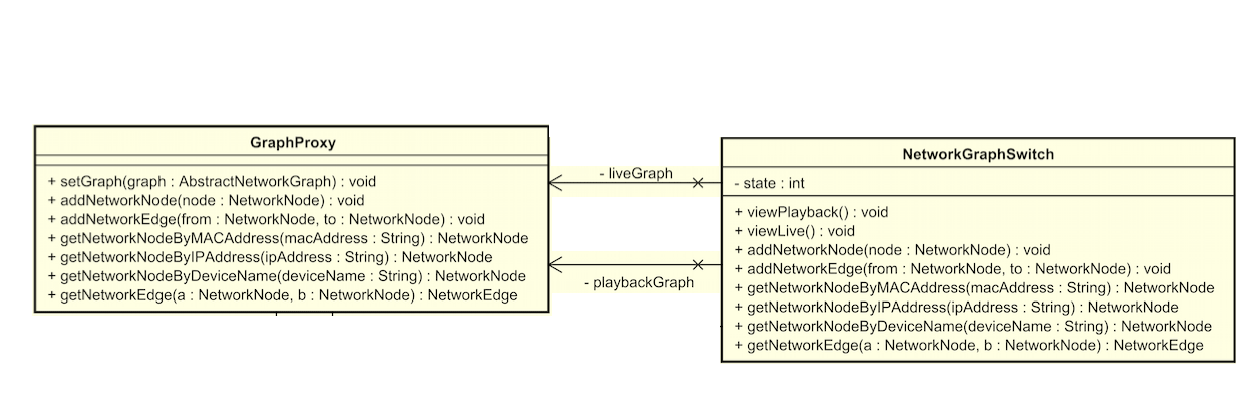
\includegraphics[width=\textwidth]{./images/graph-proxy.png}
  \end{figure}
\end{frame}

\begin{frame}{model - configdata}
  \begin{figure}
    \centering
    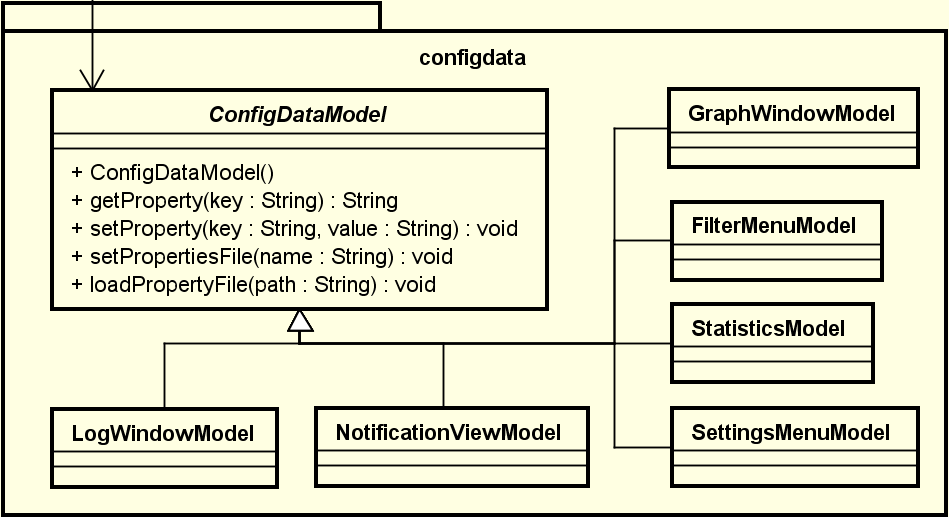
\includegraphics[width=0.7\textwidth]{./images/configdata.png}
  \end{figure}
\end{frame}


\subsection{view}
\label{subsec:view}

***view image here**

\subsection{interaction}
\label{subsec:interaction}

Dieses Package beinhaltet Enums, die die Verknüpfung zwischen Commands und Nutzerinteraktionen herstellt.
Für weitere Informationen zur Verwendung siehe \ref{subsec:view}

\begin{figure}[H]
  \centering
  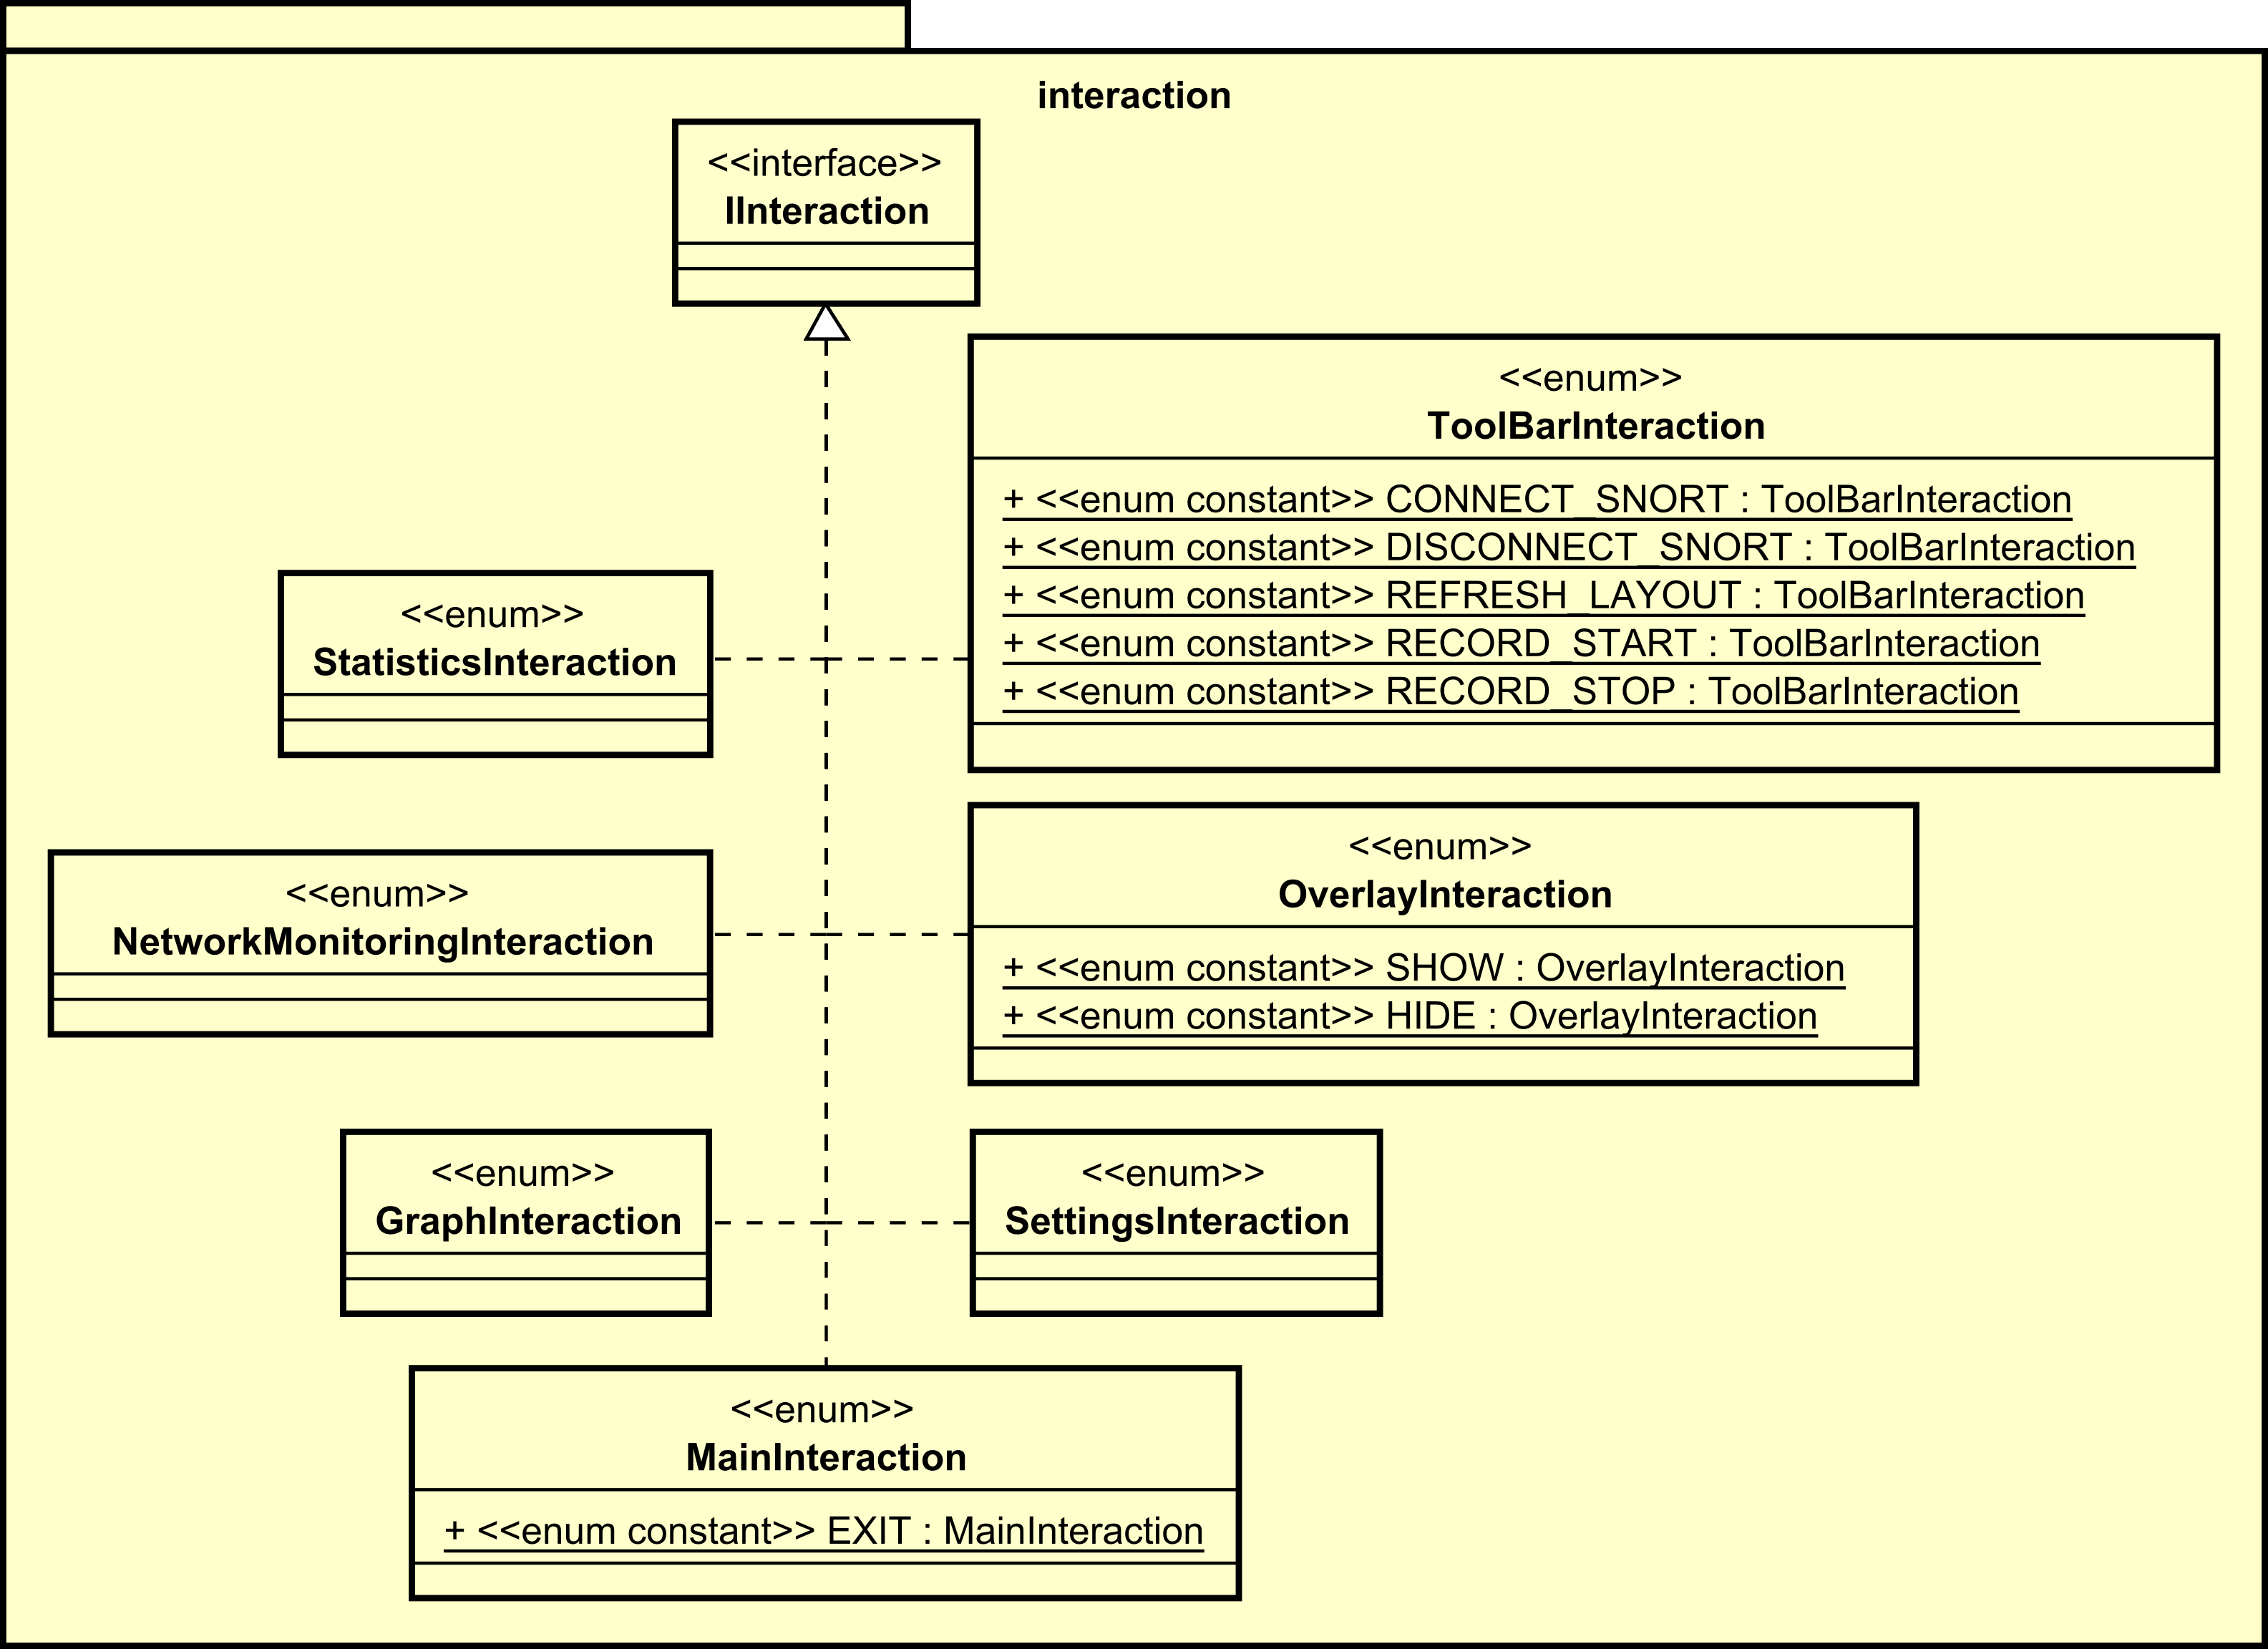
\includegraphics[width=\textwidth]{../diagramimages/interaction.png}
  \caption{interaction-Package}
\end{figure} 

\medskip
